\documentclass[12pt]{article}

\usepackage{polski}
\usepackage[utf8]{inputenc}
\usepackage{graphicx}
\usepackage{tikz}
\usepackage{amsmath}
\usepackage{epstopdf}
\usepackage{float} 
%\usepackage[colorlinks=true]{hyperref}
%\usepackage[all]{hypcap}
%\usepackage{showframe}
\usepackage{geometry}
 \geometry{
 a4paper, 
 left=30mm,
 right=30mm,
 top=30mm,
 bottom=30mm,
 }

\begin{document}

\section{Schematy}

\begin{center}
	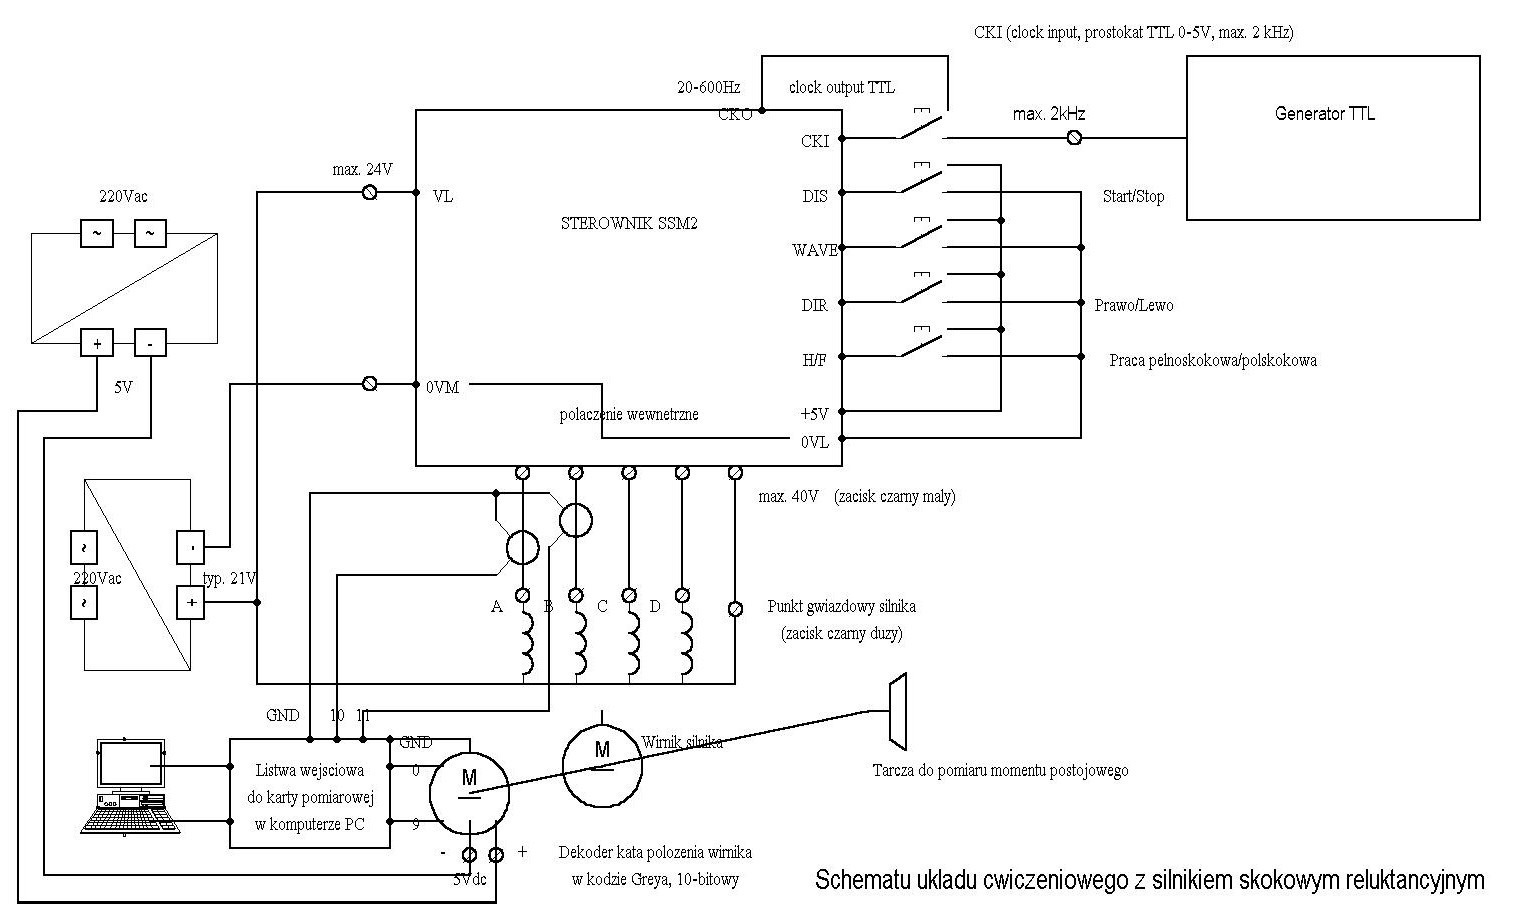
\includegraphics[height=13cm,angle=-90]{../res/img/schemat1.jpg}
\end{center}

\begin{center}
	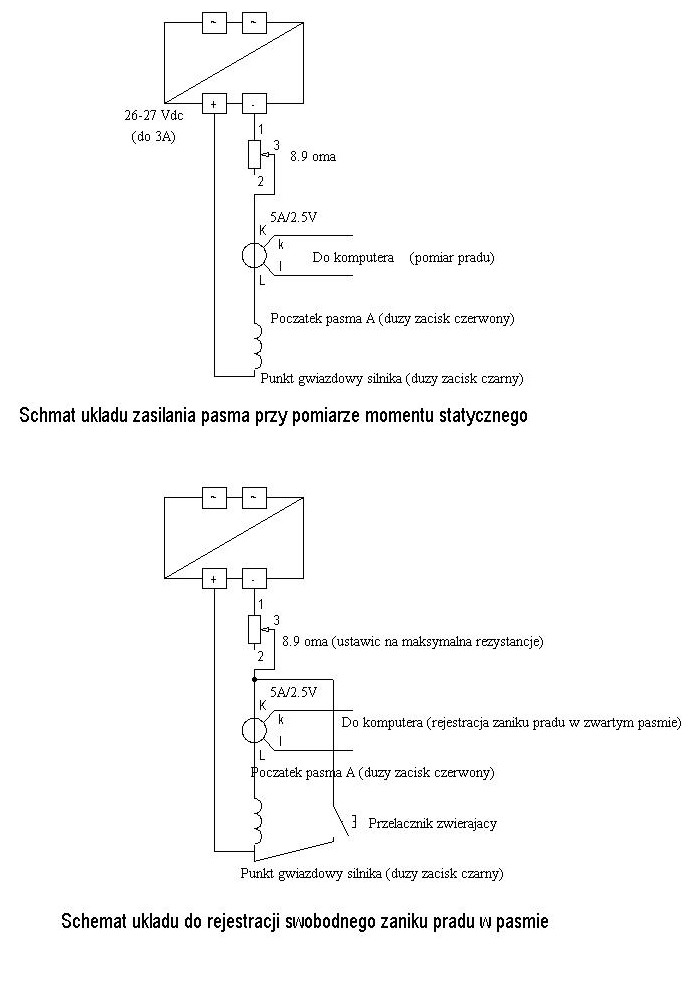
\includegraphics[width=\linewidth]{../res/img/schematy2.jpg}
\end{center}

\newpage

\section{Wyniki pomiarów i symulacji}

\begin{figure}[!htb]
	\begin{center}
		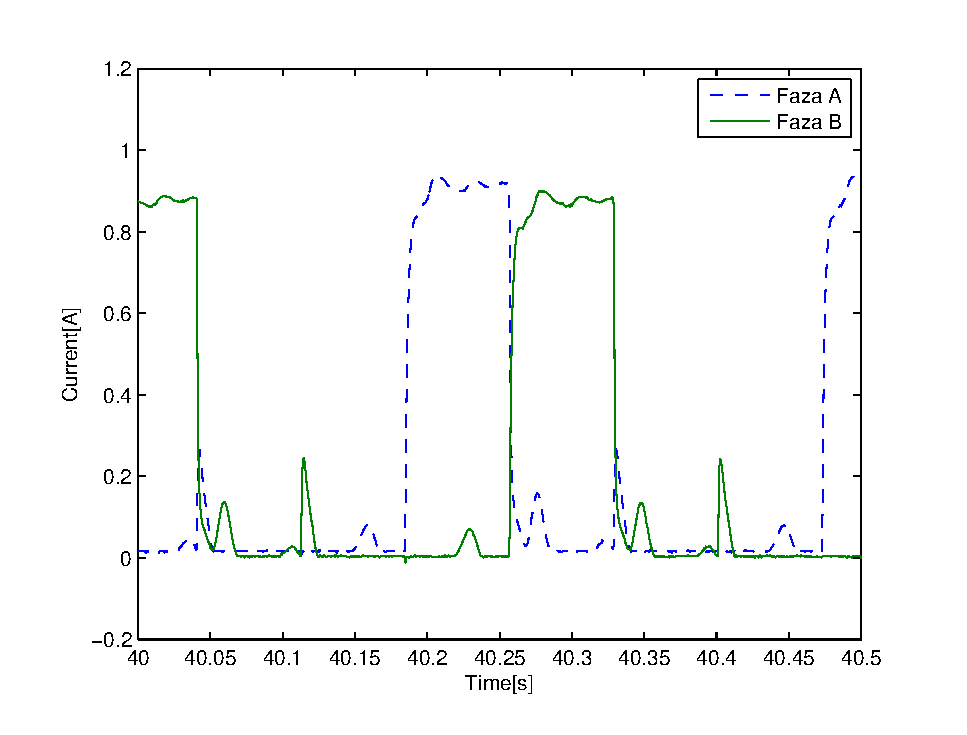
\includegraphics[width=11cm]{../res/img/pel_wol.eps}
	\end{center}
	\caption{Przebiegi prądów uzwojeń A i B dla pracy pełnokrokowej przy niskiej
	częstotliwości przełączeń}
\end{figure}
\begin{figure}[!htb]
	\begin{center}
		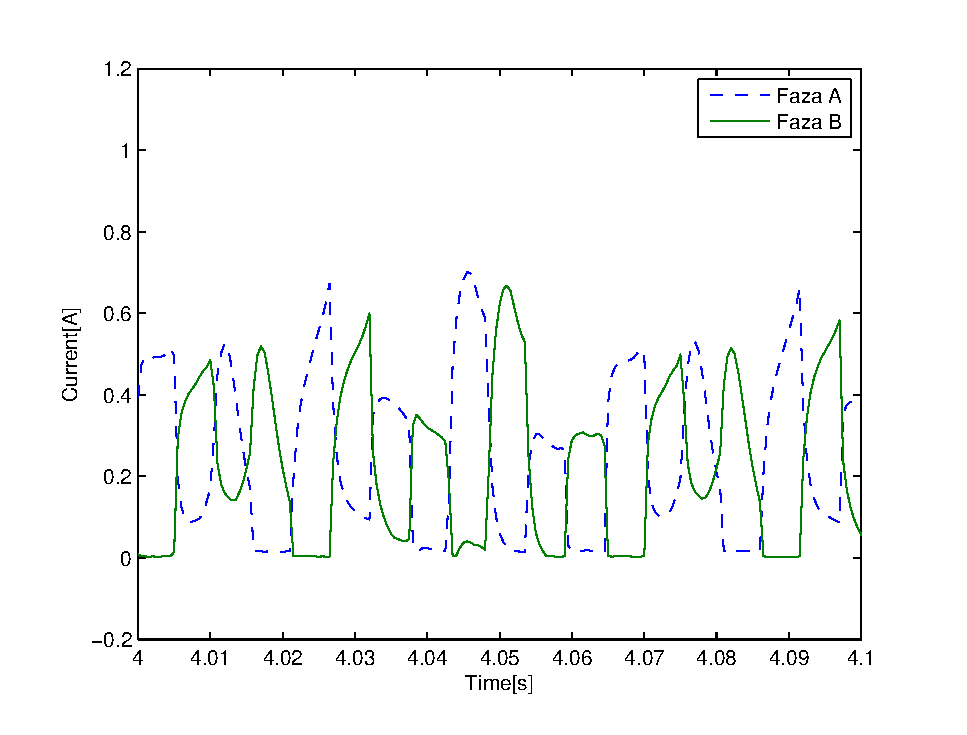
\includegraphics[width=11cm]{../res/img/pel_szyb.eps}
	\end{center}
	\caption{Przebiegi prądów uzwojeń A i B dla pracy pełnokrokowej przy
	częstotliwości przełączeń bliskiej częstotliwości granicznej}
\end{figure}

\begin{figure}[!htb]
	\begin{center}
		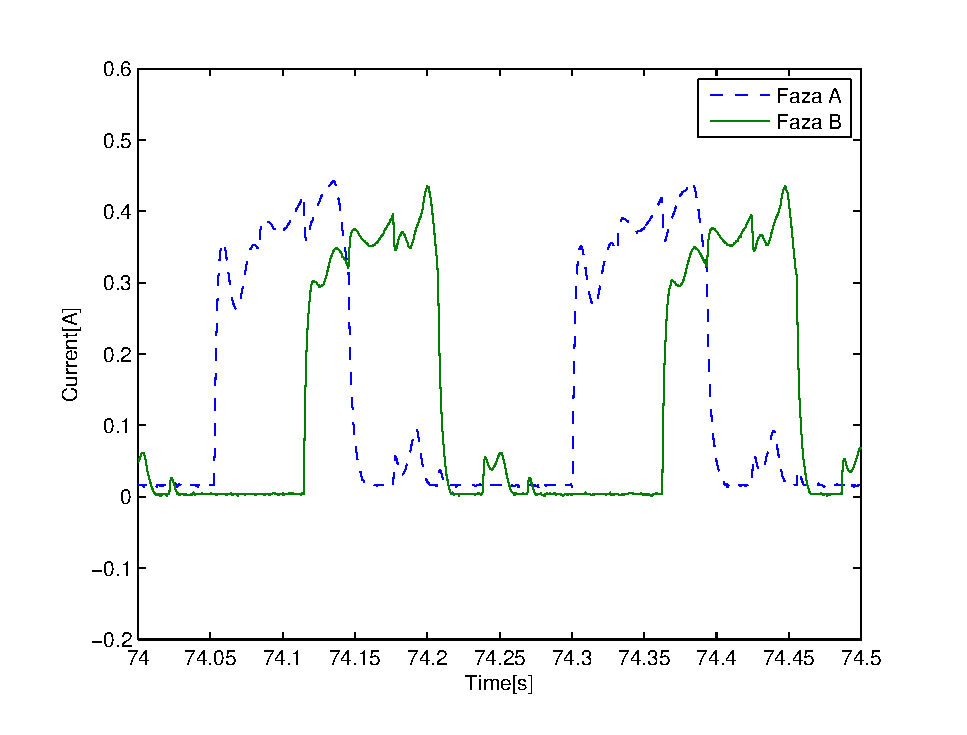
\includegraphics[width=11cm]{../res/img/pol_wol.eps}
	\end{center}
	\caption{Przebiegi prądów uzwojeń A i B dla pracy półkrokowej przy niskiej
	częstotliwości przełączeń}
\end{figure}
\begin{figure}[!htb]
	\begin{center}
		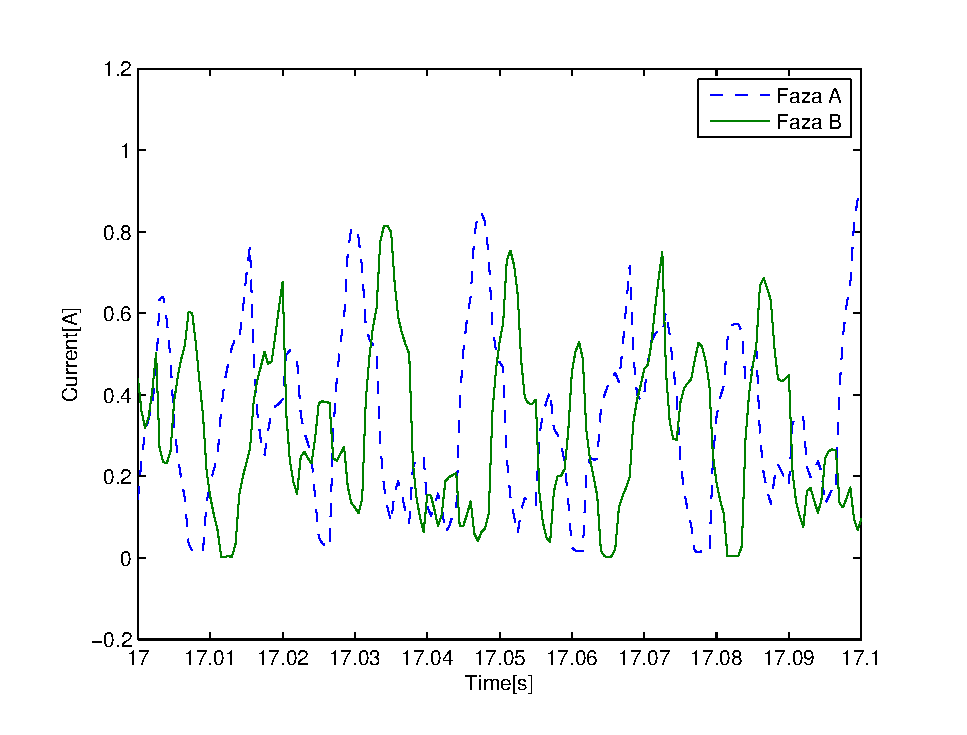
\includegraphics[width=11cm]{../res/img/pol_szyb.eps}
	\end{center}
	\caption{Przebiegi prądów uzwojeń A i B dla pracy półkrokowej przy
	częstotliwości przełączeń bliskiej częstotliwości granicznej}
\end{figure}

\begin{figure}[!htb]
	\begin{center}
		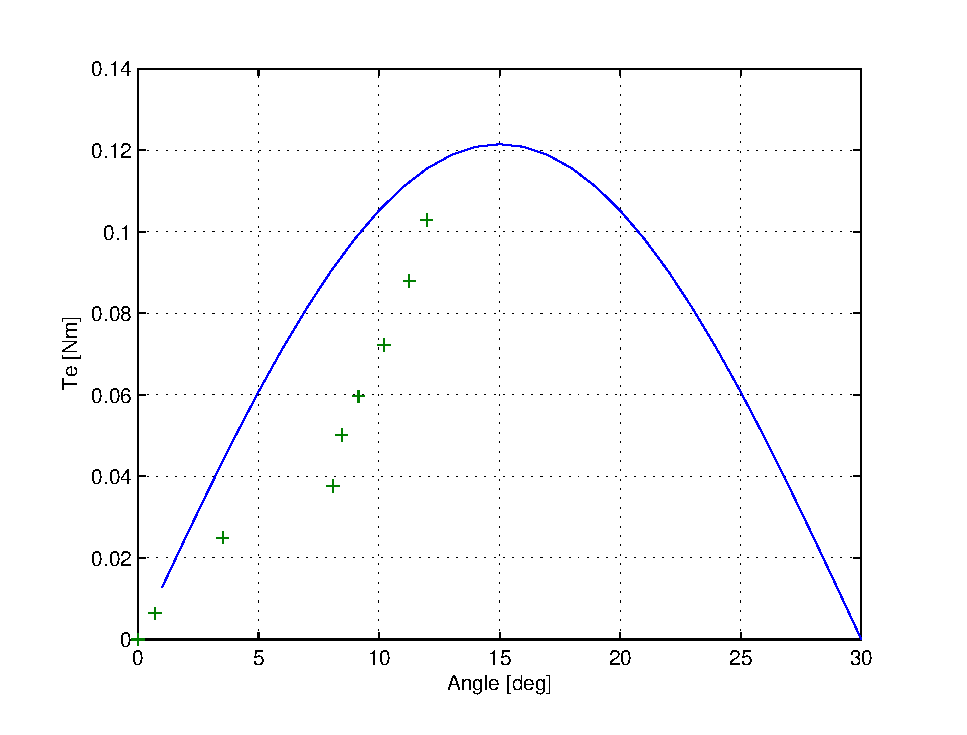
\includegraphics[width=11cm]{../res/img/mom_f-fi.eps}
	\end{center}
	\caption{Zmierzone wartości momentu postojowego silnika w funkcji kąta obrotu
	wirnika na tle zależności teoretycznej}
\end{figure}

\begin{figure}[!htb]
	\begin{center}
		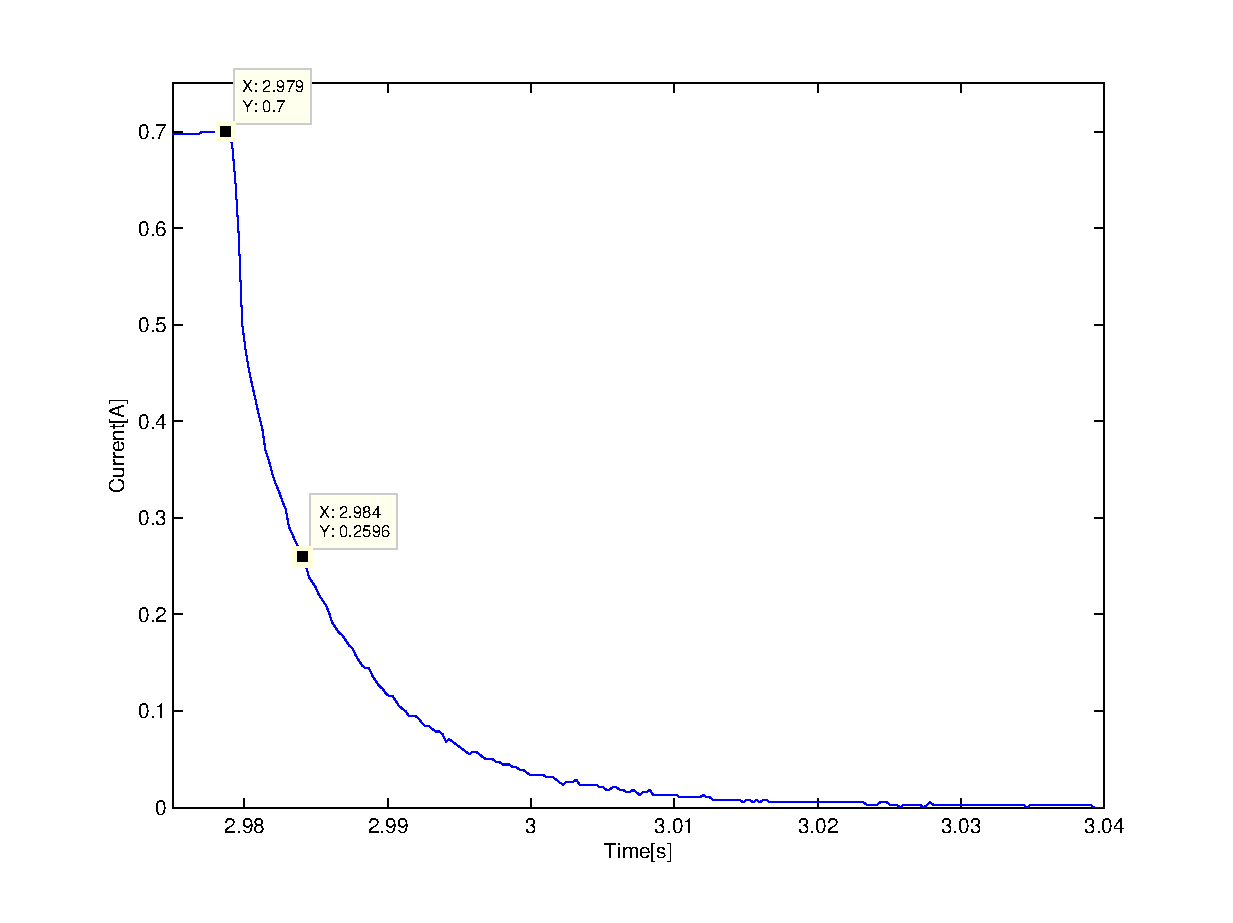
\includegraphics[width=11cm]{../res/img/Acurr.eps}
	\end{center}
	\caption{Przebieg zaniku prądu w uzwojeniu silnika po jego zwarciu}
\end{figure}

\clearpage

\section{Równania modelu silnika}

\begin{equation*}
	dL_n=-L_1Z_r\cdot \sin\left[Z_r(\varphi-n\cdot
	2\pi\cdot\frac{1}{Z_s})\right],\hspace{0.5cm} n=0,1,2,3
\end{equation*}

\begin{equation*}
	L_n=L_0+L_1\cdot \cos\left[Z_r(\varphi-n\cdot
	2\pi\cdot\frac{1}{Z_s})\right],\hspace{0.5cm} n=0,1,2,3
\end{equation*}

\begin{equation*}
	di_n=\frac{U_n-R\cdot i_n-dL_n\cdot\omega\cdot i_n}{L_n}\hspace{0.5cm}
	n=0,1,2,3
\end{equation*}

\begin{equation*}
	T_e=\frac{1}{2}(dL_0\cdot i_0^2+dL_1\cdot i_1^2+dL_2\cdot i_2^2+dL_3\cdot
	i_3^2)
\end{equation*}

\begin{equation*}
	d\omega=\frac{T_e-D\omega+T_z}{I}
\end{equation*}

\begin{equation*}
	d\varphi=\omega
\end{equation*}

\end{document}
